\documentclass[a4paper]{article}
\usepackage[T1]{fontenc}
\usepackage[russian]{babel}
\usepackage[pdftex]{graphicx}
\usepackage[ruled,vlined]{algorithm2e}
\usepackage[utf8]{inputenc}
\usepackage{xcolor}
\usepackage{hyperref}
\usepackage{amsmath}
\usepackage{geometry}
\usepackage{float}
\usepackage{caption}
\usepackage{subcaption}
\DeclareGraphicsExtensions{.pdf,.png,.jpg}

\begin{document}

    \begin{titlepage}
        \Large
        \begin{center}
            Санкт-Петербургский \ Политехнический университет Петра Великого\\
            \vspace{10em}Отчет по лабораторной работе №3\\
            \vspace{2em}
            \textbf{Анализ выбросов в распределениях}
        \end{center}
        \vspace{6em}
        \hfill\parbox{10cm}{
            \hspace*{2cm}\hspace*{-4cm}Студент:\hfill Швачко Никита Андреевич\\
            \hspace*{2cm}\hspace*{-4cm}Преподаватель:\hfill Баженов Александр Николаевич\\
            \hspace*{2cm}\hspace*{-4cm}Группа:\hfill 5030102/20202
        }
        \vspace{\fill}
        \begin{center}
            Санкт-Петербург \ 2025
        \end{center}
    \end{titlepage}


    \section{Формулировка задания и его формализация}\label{sec:task}
    Для анализа двухмерных нормальных распределений и смесей нормальных распределений необходимо:
    \begin{enumerate}
        \item Сгенерировать выборки размерами 20, 60 и 100 элементов для нормального двумерного распределения $N(x, y, 0,0,1,1,\rho)$ с коэффициентами корреляции $\rho = 0.0, 0.5, 0.9$.
        \item Каждая выборка генерируется 1000 раз, после чего вычисляются следующие статистики:
        \begin{itemize}
            \item Среднее значение для коэффициентов корреляции Пирсона, Спирмена и квадрантного коэффициента корреляции.
            \item Среднее значение квадрата этих коэффициентов.
            \item Дисперсия этих коэффициентов.
        \end{itemize}
        \item Повторить все вычисления для смеси нормальных распределений:
        $$f(x, y) = 0.9 N(x, y, 0,0,1,1,0.9) + 0.1 N(x, y, 0,0,10,10,-0.9)$$
        \item Изобразить сгенерированные точки на плоскости и нарисовать эллипс равновероятности для каждого случая.
    \end{enumerate}


    \section{Сгенерированные точки и эллипсы равновероятности}\label{sec:scatterplots}
    Для каждой выборки была выполнена генерация точек и построение эллипсов равновероятности. Ниже представлены графики сгенерированных точек для различных коэффициентов корреляции.

    \begin{figure}[H]
        \centering
        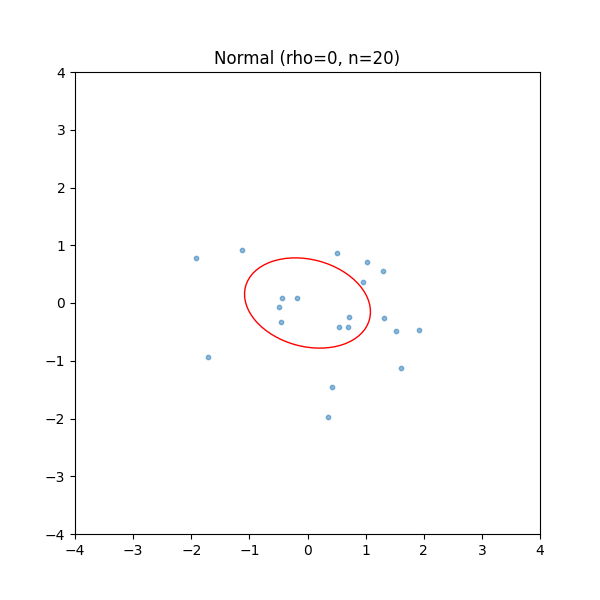
\includegraphics[width=0.8\textwidth]{./plots/normal_rho0_n20}
        \caption{Генерация точек для $\rho = 0.0$ и эллипс равновероятности для $n=20$}
        \label{fig:normal_rho0_n20}
    \end{figure}

    \begin{figure}[H]
        \centering
        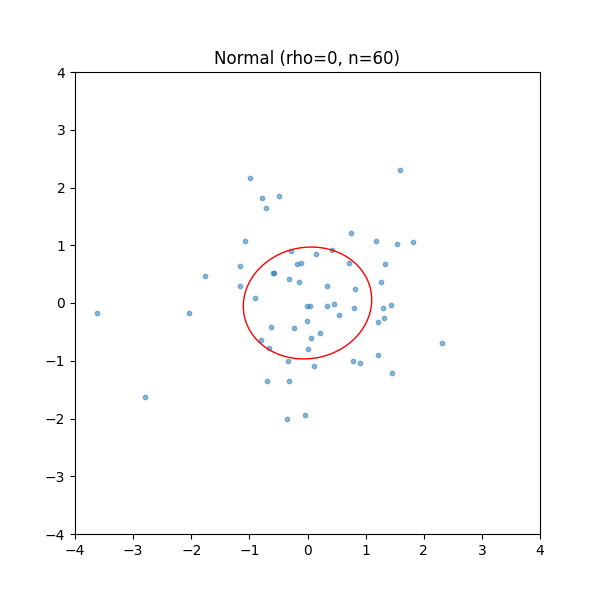
\includegraphics[width=0.8\textwidth]{./plots/normal_rho0_n60}
        \caption{Генерация точек для $\rho = 0.0$ и эллипс равновероятности для $n=60$}
        \label{fig:normal_rho0_n60}
    \end{figure}

    \begin{figure}[H]
        \centering
        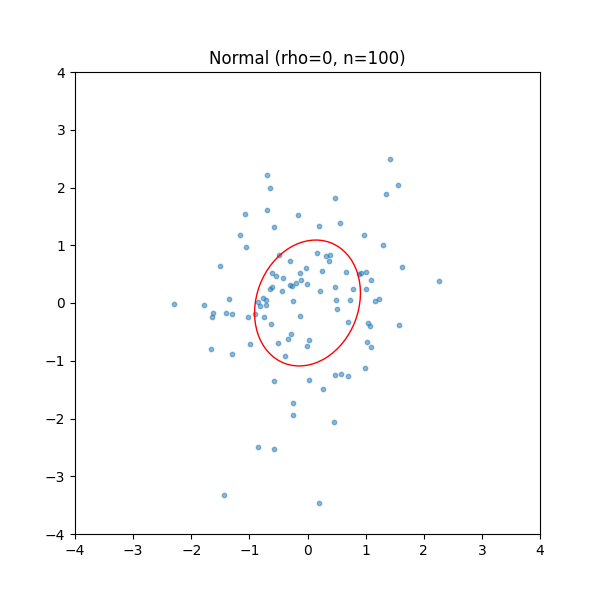
\includegraphics[width=0.8\textwidth]{./plots/normal_rho0_n100}
        \caption{Генерация точек для $\rho = 0.0$ и эллипс равновероятности для $n=100$}
        \label{fig:normal_rho0_n100}
    \end{figure}

    \begin{figure}[H]
        \centering
        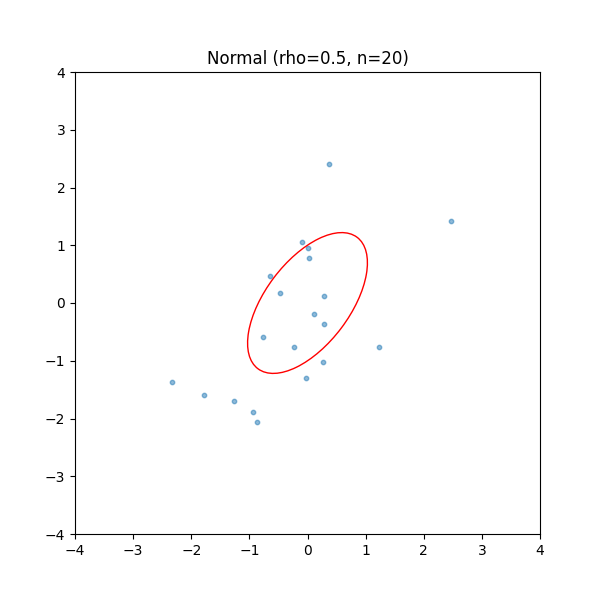
\includegraphics[width=0.8\textwidth]{./plots/normal_rho0.5_n20}
        \caption{Генерация точек для $\rho = 0.5$ и эллипс равновероятности для $n=20$}
        \label{fig:normal_rho0.5_n20}
    \end{figure}

    \begin{figure}[H]
        \centering
        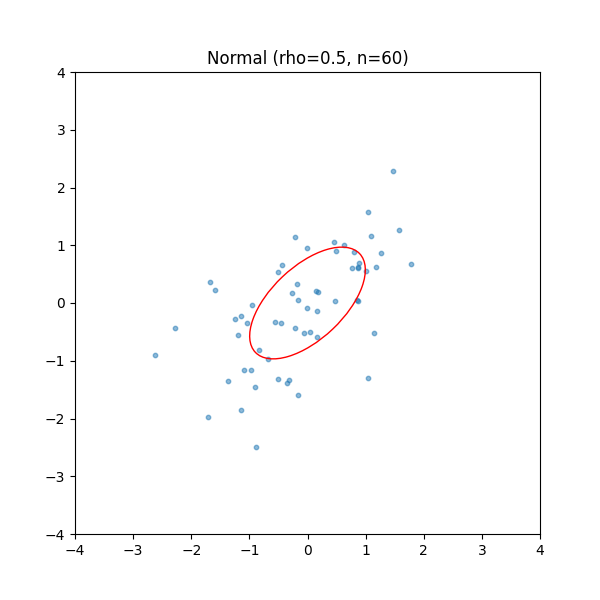
\includegraphics[width=0.8\textwidth]{./plots/normal_rho0.5_n60}
        \caption{Генерация точек для $\rho = 0.5$ и эллипс равновероятности для $n=60$}
        \label{fig:normal_rho0.5_n60}
    \end{figure}

    \begin{figure}[H]
        \centering
        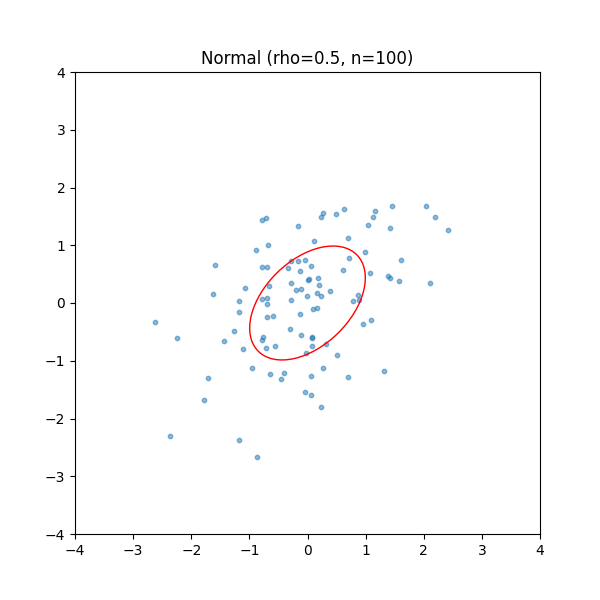
\includegraphics[width=0.8\textwidth]{./plots/normal_rho0.5_n100}
        \caption{Генерация точек для $\rho = 0.5$ и эллипс равновероятности для $n=100$}
        \label{fig:normal_rho0.5_n100}
    \end{figure}

    \begin{figure}[H]
        \centering
        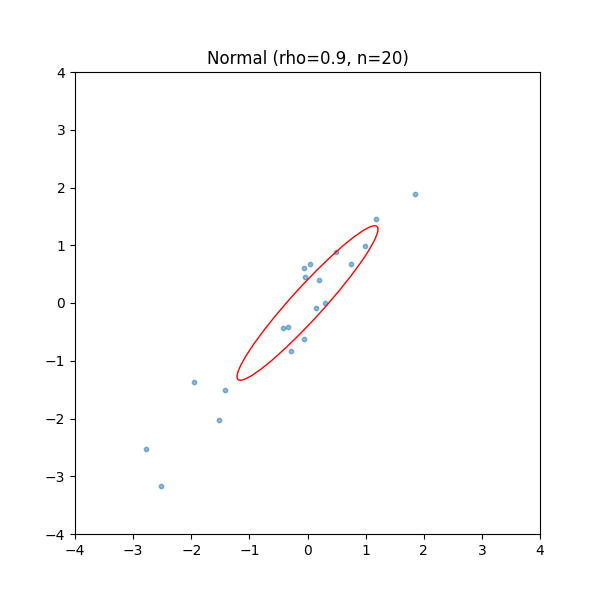
\includegraphics[width=0.8\textwidth]{./plots/normal_rho0.9_n20}
        \caption{Генерация точек для $\rho = 0.9$ и эллипс равновероятности для $n=20$}
        \label{fig:normal_rho0.9_n20}
    \end{figure}

    \begin{figure}[H]
        \centering
        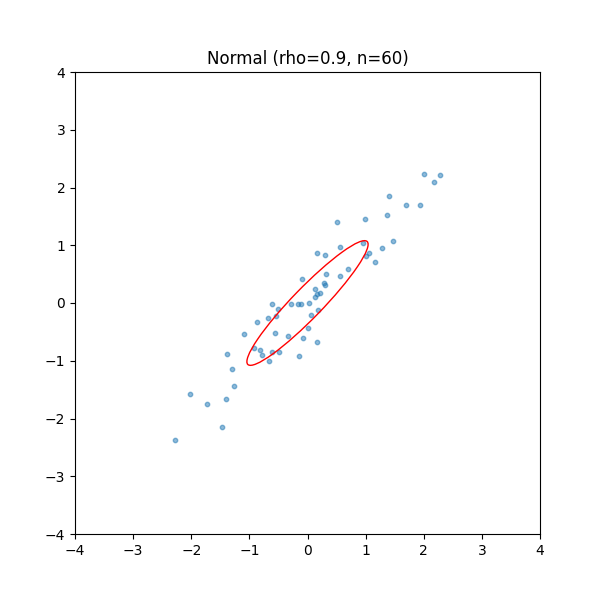
\includegraphics[width=0.8\textwidth]{./plots/normal_rho0.9_n60}
        \caption{Генерация точек для $\rho = 0.9$ и эллипс равновероятности для $n=60$}
        \label{fig:normal_rho0.9_n60}
    \end{figure}

    \begin{figure}[H]
        \centering
        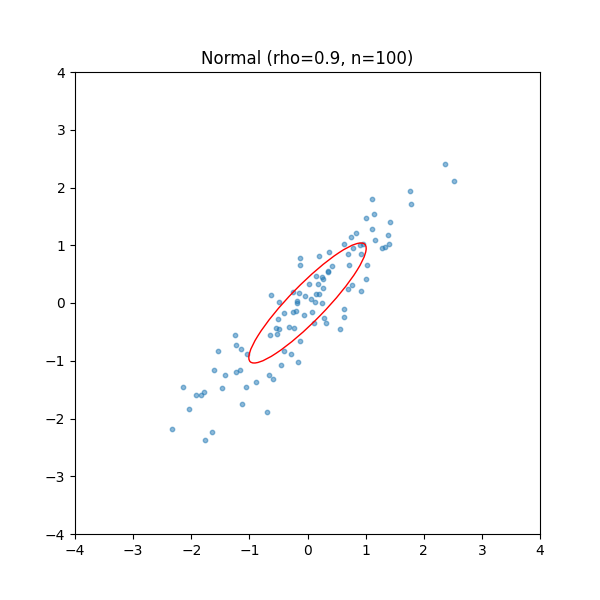
\includegraphics[width=0.8\textwidth]{./plots/normal_rho0.9_n100}
        \caption{Генерация точек для $\rho = 0.9$ и эллипс равновероятности для $n=100$}
        \label{fig:normal_rho0.9_n100}
    \end{figure}


    \section{Результаты для смеси нормальных распределений}\label{sec:mixture_results}
    Также были выполнены вычисления для смеси нормальных распределений. Графики точек и эллипсов равновероятности для смеси представлены ниже.

    \begin{figure}[H]
        \centering
        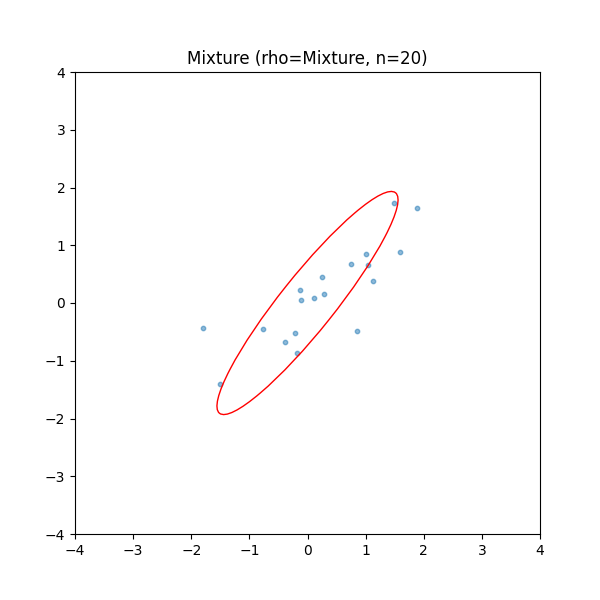
\includegraphics[width=0.8\textwidth]{./plots/mixture_rhoMixture_n20}
        \caption{Генерация точек для смеси с эллипсом равновероятности для $n=20$}
        \label{fig:mixture_rhoMixture_n20}
    \end{figure}

    \begin{figure}[H]
        \centering
        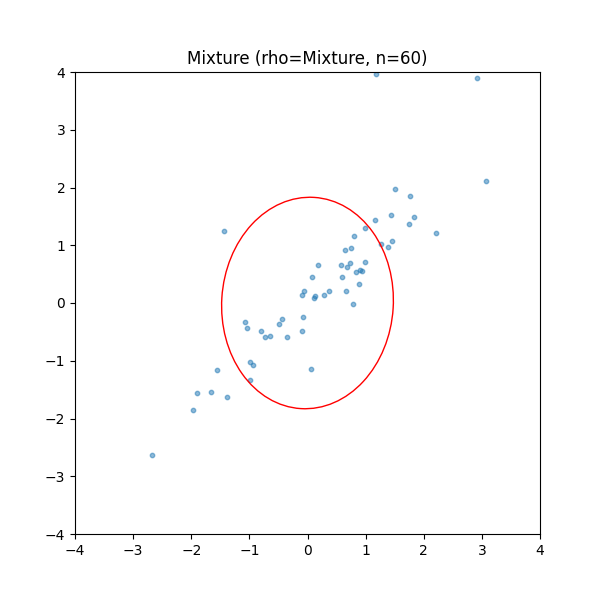
\includegraphics[width=0.8\textwidth]{./plots/mixture_rhoMixture_n60}
        \caption{Генерация точек для смеси с эллипсом равновероятности для $n=60$}
        \label{fig:mixture_rhoMixture_n60}
    \end{figure}

    \begin{figure}[H]
        \centering
        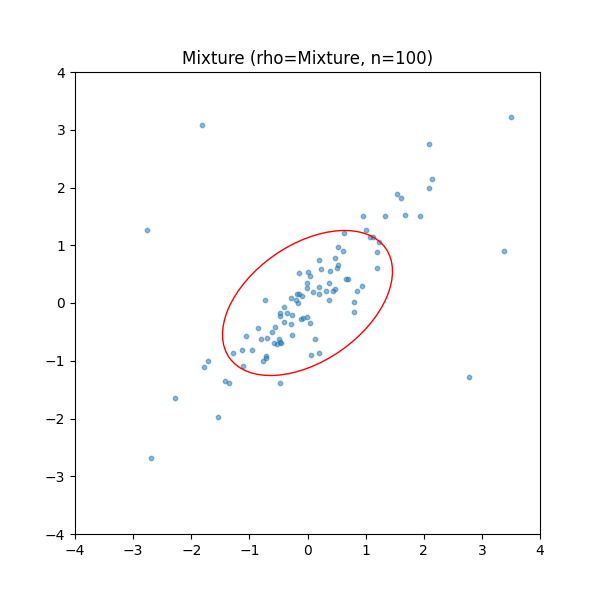
\includegraphics[width=0.8\textwidth]{./plots/mixture_rhoMixture_n100}
        \caption{Генерация точек для смеси с эллипсом равновероятности для $n=100$}
        \label{fig:mixture_rhoMixture_n100}
    \end{figure}


    \section{Результаты вычислений для коэффициентов корреляции}\label{sec:correlation_results}
    В результате вычислений для каждого коэффициента корреляции были получены следующие статистики (среднее значение, среднее квадрата и дисперсия) для выборок размером 20, 60 и 100.
    \begin{table}[!htbp]
        \caption{Средние значения и дисперсии коэффициентов корреляции для различных выборок}
        \label{tab:correlation_results}
        \noindent
        \resizebox{\textwidth}{!}{
            \begin{tabular}{|c|c|c|c|c|}
                \hline
                \textbf{Распределение, коэфф корр, размер выборки} & \textbf{Фактический коэфф корр} & \textbf{Пирсона} & \textbf{Спирмена} & \textbf{Квадрантный} \\
                \hline
                ('Normal', 0, 20)                                  & -0.19                           & -0.18            & -0.23             & -0.29 \\
                ('Normal', 0, 60)                                  & 0.06                            & 0.05             & 0.01              & -0.13 \\
                ('Normal', 0, 100)                                 & 0.12                            & 0.12             & 0.08              & 0.02 \\
                ('Normal', 0.5, 20)                                & 0.47                            & 0.47             & 0.43              & 0.59 \\
                ('Normal', 0.5, 60)                                & 0.59                            & 0.59             & 0.60              & 0.54 \\
                ('Normal', 0.5, 100)                               & 0.50                            & 0.51             & 0.51              & 0.32 \\
                ('Normal', 0.9, 20)                                & 0.90                            & 0.90             & 0.82              & 0.90 \\
                ('Normal', 0.9, 60)                                & 0.95                            & 0.95             & 0.94              & 0.84 \\
                ('Normal', 0.9, 100)                               & 0.91                            & 0.91             & 0.90              & 0.70 \\
                ('Mixture', '', 20)                                & 0.45                            & 0.52             & 0.67              & 0.70 \\
                ('Mixture', '', 60)                                & 0.03                            & 0.11             & 0.63              & 0.73 \\
                ('Mixture', '', 100)                               & 0.44                            & 0.44             & 0.66              & 0.60                 \\
                \hline
            \end{tabular}
        }
    \end{table}


    \section{Выводы}\label{sec:conclusions}
    \begin{itemize}
        \item Коэффициент корреляции Пирсона, Спирмена и квадрантный коэффициент дают схожие результаты для нормального распределения с высоким коэффициентом корреляции.
        \item Для смеси нормальных распределений результаты отличаются из-за смешанных компонент с различной корреляцией.
        \item Графики и эллипсы равновероятности демонстрируют изменение зависимости между переменными в зависимости от значения коэффициента корреляции.
    \end{itemize}

\end{document}